
\documentclass[11pt,a4paper,UTF8]{book}

\usepackage{minted}
\usepackage[T1]{fontenc}
\usepackage[utf8]{inputenc}
\usepackage{authblk}

\usepackage{fontspec}                  %引入字体设置宏包
\setmainfont{Times New Roman}             %设置英文正文字体
% Courier New
% Book Antique
\setsansfont{Arial}                    %英文无衬线字体
\setmonofont{Courier New}              %英文等宽字体

\usepackage{ctex} %导入中文包
%\usepackage{ulem}
\usepackage{tocvsec2}
\usepackage{verbatim}

\usepackage{tabularx}
\usepackage{longtable}
\usepackage{booktabs} 
\usepackage{multirow}
\usepackage{bbding}
\usepackage{float}
\usepackage{xspace}
\usepackage[none]{hyphenat}

\usepackage{graphicx}
\usepackage{subfigure}
\usepackage{pifont}

\usepackage{hyperref}  %制作pdf的目录
\usepackage{subfiles} %使用多文件方式进行

\usepackage{geometry} %设置页边距的包
\geometry{left=2.5cm,right=2cm,top=2.54cm,bottom=2.54cm} %设置书籍的页边距

\usepackage{url}
\hypersetup{hidelinks, %去红框
	colorlinks=true,
	allcolors=black,
	pdfstartview=Fit,
	breaklinks=true
}

% 调整itemlist中的行间距
\usepackage{enumitem}
\setenumerate[1]{itemsep=0pt,partopsep=0pt,parsep=\parskip,topsep=5pt}
\setitemize[1]{itemsep=0pt,partopsep=0pt,parsep=\parskip,topsep=5pt}
\setdescription{itemsep=0pt,partopsep=0pt,parsep=\parskip,topsep=5pt}

% 超链接样式设置
\usepackage{hyperref}
\hypersetup{
	colorlinks=true,
	linkcolor=blue,
	filecolor=blue,
	urlcolor=blue,
	citecolor=cyan,
}

\usepackage{indentfirst}

\usepackage{listings}
\usepackage[usenames,dvipsnames,svgnames, x11names]{xcolor}

\usepackage[most]{tcolorbox}
\tcbuselibrary{breakable} % 引入 breakable 库
\tcbuselibrary{skins} % 引入 skins 库

%定义CMake
\lstdefinelanguage{CMake}
{morekeywords={
		cmake\_minimum\_required,
		project,
		add\_executable,
		add\_library,
		target\_link\_libraries,
		cmake\_parse\_arguments,
		cmake\_language,
		set, unset,
		option,
		string,
		list,
		math,
		message,
		if, elseif, else, endif,
		mark\_as\_advanced,
		foreach, endforeach,
		while, endwhile,
		add\_subdirectory, include, return, include\_gurad,
		function, endfunction,
		macro, endmacro,
		find\_package,
		cmake\_push\_check\_state,
		cmake\_pop\_check\_state,
		cmake\_reset\_check\_state,
		add\_test,
		set\_tests\_properties, 
		check\_c\_source\_runs,
		check\_cxx\_source\_runs,
		check\_fortran\_source\_runs,
		check\_source\_runs,
		check\_compiler\_flag,
		check\_c\_compiler\_flag,
		check\_cxx\_compiler\_flag,
		check\_fortran\_compiler\_flag,
		check\_symbol\_exists,
		check\_cxx\_symbol\_exists,
		check\_linker\_flag,
		cmake\_policy,
		set\_property,
		get\_property,
		define\_property,
		get\_cmake\_property,
		set\_cmake\_property,
		set\_target\_properties,
		get\_target\_property,
		set\_directory\_properties,
		get\_directory\_property,
		set\_source\_files\_properties,
		get\_source\_file\_property,
		set\_tests\_properties,
		get\_tests\_property,
		get\_test\_property,
		cmake\_print\_properties,
		cmake\_print\_variables,
		variable\_watch,
		include\_guard,
		target\_link\_options,
		target\_compile\_definitions,
		target\_compile\_options,
		include\_directories,
		add\_definitions,
		remove\_definitions,
		add\_compile\_definitions,
		add\_compile\_options,
		link\_libraries,
		link\_directories,
		add\_link\_options,
		target\_include\_directories,
		target\_compile\_features,
		add\_custom\_command,
		add\_custom\_target,
		execute\_process,
		cmake\_path,
		get\_filename\_component,
		file,
		configure\_file,
		generate\_export\_header,
		export,
		find\_file,
		find\_library,
		find\_package,
		find\_program,
		pkg\_check\_modules,
		pkg\_search\_module,
		pkg\_get\_variable,
		add\_test,
		enable\_testing,
		set\_tests\_properties,
		site\_name,
		ctest\_empty\_binary\_directory,
		ctest\_start,
		ctest\_configure,
		ctest\_submit,
		ctest\_build,
		ctest\_memcheck,
		ctest\_upload,
		ctest\_test,
		gtest\_add\_tests,
		gtest\_discover\_tests,
		install,
		write\_basic\_package\_version\_file,
		configure\_package\_config\_file,
		cpack\_add\_component,
		cpack\_add\_install\_type,
		cpack\_add\_component\_group,
		ExternalProject\_Add,
		ExternalProject\_Add\_StepDependencies,
		ExternalProject\_Get\_Property,
		ExternalProject\_Add\_Step,
		FetchContent\_Declare,
		FetchContent\_GetProperties,
		FetchContent\_Populate,
		source\_group,
		target\_precompile\_headers,
		qt5\_wrap\_cpp,
		qt5\_wrap\_ui,
		qt5\_add\_resources,
		qt5\_add\_big\_resources,
		qt5\_add\_binary\_resources,
		qt5\_add\_translation,
		qt5\_create\_translation,
		compile\_definitions,
		add\_llvm\_component\_library,
		add\_llvm\_tool,
		llvm\_multisource,
		llvm\_test\_data,
		doxygen\_add\_docs,
		cmake\_dependent\_option,
		target\_sources,
		conan\_cmake\_autodetect,
		conan\_cmake\_configure,
		conan\_cmake\_install,
		doxygen\_add\_docs,
		check\_source\_compiles,
		check\_language,
		enable\_language,
		add\_dependencies,
		find\_path,
		find\_package\_handle\_standard\_args,
	}, %定义关键字
	sensitive=false, %是否大小写敏感
	morecomment=[l]{\#},
	morestring=[b]",
	morestring=[d]',
}

\lstdefinestyle{styleCMake}{
	language=CMake,
	backgroundcolor=\color{blue!3!white}, 
	basicstyle=\tt, 
	breakatwhitespace = false,
	breaklines = true,
	captionpos = b,
	commentstyle = \color{mygray}\bfseries, 
	extendedchars =false,             
	frame=shadowbox, 
	tabsize=2,
	framerule=0.5pt,
	keepspaces=true,
	keywordstyle=\color{blue}\bfseries, % keyword style
	otherkeywords={string}, 
	rulecolor=\color{black},
	showspaces=false,
	showstringspaces=false,
	showtabs=false,
	stepnumber=1,
	stringstyle=\color{purple},        % string literal style
}

\lstdefinestyle{stylePython}{
	language        =   Python, % 语言选Python
	backgroundcolor=\color{blue!3!white}, 
	basicstyle      =   \zihao{-5}\ttfamily,
	numberstyle     =   \zihao{-5}\ttfamily,
	keywordstyle    =   \color{blue},
	keywordstyle    =   [2] \color{teal},
	stringstyle     =   \color{magenta},
	commentstyle    =   \color{red}\ttfamily,
	frame = shadowbox, 
	breaklines      =   true,   % 自动换行,建议不要写太长的行
	columns         =   fixed,  % 如果不加这一句,字间距就不固定,很丑,必须加
	basewidth       =   0.5em,
	%basicstyle          =   \sffamily,          % 基本代码风格
	%keywordstyle        =   \bfseries,          % 关键字风格
	%commentstyle        =   \rmfamily\itshape,  % 注释的风格,斜体
	%stringstyle         =   \ttfamily,  % 字符串风格
	flexiblecolumns,                % 别问为什么,加上这个
	%numbers             =   left,   % 行号的位置在左边
	showspaces          =   false,  % 是否显示空格,显示了有点乱,所以不现实了
	numberstyle         =   \zihao{-5}\ttfamily,    % 行号的样式,小五号,tt等宽字体
	showstringspaces    =   false,
	captionpos          =   t,      % 这段代码的名字所呈现的位置,t指的是top上面
	frame               =   lrtb,   % 显示边框
	tabsize=2,  
}

\tcbset{
	breakable,
	commandshell/.style={
		listing only,
		colback=black!75!white,
		colupper=white,
		lowerbox=ignored,
		listing options={
			language={bash},
			breaklines=true,
			basicstyle=\ttfamily,
			columns = fixed,
			flexiblecolumns
		}
}}

\usepackage{tikz}

% URL 正确换行
% https://liam.page/2017/05/17/help-the-url-command-from-hyperref-to-break-at-line-wrapping-point/
\makeatletter
\def\UrlAlphabet{%
	\do\a\do\b\do\c\do\d\do\e\do\f\do\g\do\h\do\i\do\j%
	\do\k\do\l\do\m\do\n\do\o\do\p\do\q\do\r\do\s\do\t%
	\do\u\do\v\do\w\do\x\do\y\do\z\do\A\do\B\do\C\do\D%
	\do\E\do\F\do\G\do\H\do\I\do\J\do\K\do\L\do\M\do\N%
	\do\O\do\P\do\Q\do\R\do\S\do\T\do\U\do\V\do\W\do\X%
	\do\Y\do\Z}
\def\UrlDigits{\do\1\do\2\do\3\do\4\do\5\do\6\do\7\do\8\do\9\do\0}
\g@addto@macro{\UrlBreaks}{\UrlOrds}
\g@addto@macro{\UrlBreaks}{\UrlAlphabet}
\g@addto@macro{\UrlBreaks}{\UrlDigits}
\makeatother

% enable subsubsubsection
% from https://tex.stackexchange.com/练习题/274212/correct-hierarchy-levels-of-pdf-bookmarks-for-custom-section-subsubsubsection
\usepackage[depth=3]{bookmark}
\setcounter{secnumdepth}{3}
\setcounter{tocdepth}{4}
\hypersetup{bookmarksdepth=4}

\makeatletter

\newcommand{\toclevel@subsubsubsection}{4}
\newcounter{subsubsubsection}[subsubsection]

\renewcommand{\thesubsubsubsection}{\thesubsubsection.\arabic{subsubsubsection}}

\newcommand{\subsubsubsection}{\@startsection{subsubsubsection}{4}{\z@}%
	{-3.25ex\@plus -1ex \@minus -.2ex}%
	{1.5ex \@plus .2ex}%
	{\normalfont\normalsize\bf\bfseries}}

\newcommand*{\l@subsubsubsection}{\@dottedtocline{4}{11em}{5em}}  

\newcommand{\subsubsubsectionmark}[1]{}
\makeatother

\ExplSyntaxOn

% Setup enumerate, itemize and description
\setenumerate  { nosep }
\setitemize    { nosep }
\setdescription{ nosep }

% Setup minted
\setminted { obeytabs, tabsize=2, breaklines=true, fontsize=\footnotesize, frame=single }

% Def \filename
\NewDocumentCommand { \filename } { m } 
{ \noindent \textit { #1 } \vspace*{ -1ex } \nopagebreak[4] }

% Def \mySamllsection
\NewDocumentCommand { \mySamllsection } { m } 
{ \noindent \hspace*{\fill} \\ \textbf { #1 } \vspace*{ -1ex } \nopagebreak[4] \\ }

% Def \inlcpp
\NewDocumentCommand { \inlcpp }   { m } 
{ \mintinline { cpp } { #1 } }

% Def cpp environment
\NewDocumentEnvironment { cpp } { }
{ \VerbatimEnvironment
	\begin { minted } [ linenos=true ] { cpp } } 
{ \end   { minted } }

% Def shell environment
\NewDocumentEnvironment { shell } { }
{ \VerbatimEnvironment
	\begin { minted } { text } } 
{ \end   { minted } }

\NewDocumentEnvironment { notice } { }
{ \begin { tcolorbox } [ colback = green!5!white, colframe=green!75!black ] } 
{ \end   { tcolorbox } }

\NewDocumentCommand { \mySubsubsection } { mm }
{ 
\subsubsection*{\zihao{3} {#1} \hspace{0.2cm}{#2}}
\addcontentsline{toc}{subsubsection}{{#1}\hspace{0.2cm}{#2}}
}

\NewDocumentCommand { \mySubsection } { mmm }
{
\subsection*{\zihao{3}{#1}\hspace{0.2cm}{#2}}
\addcontentsline{toc}{subsection}{{#1}\hspace{0.2cm}{#2}}
\subfile{{#3}}
}

\NewDocumentCommand { \mySection } { mmm }
{
\section*{\zihao{2}{#1}\hspace{0.5cm}{#2}}
\addcontentsline{toc}{section}{{#1}\hspace{0.5cm}{#2}}
\subfile{{#3}}
}

% Latex如何在文本模式批量处理下划线
% https://zhuanlan.zhihu.com/p/615108006 

\ExplSyntaxOff

\begin{document}
	\begin{sloppypar} %latex中一行文字出现溢出问题的解决方法
		%\maketitle
		
		\begin{center}
			\thispagestyle{empty}
			%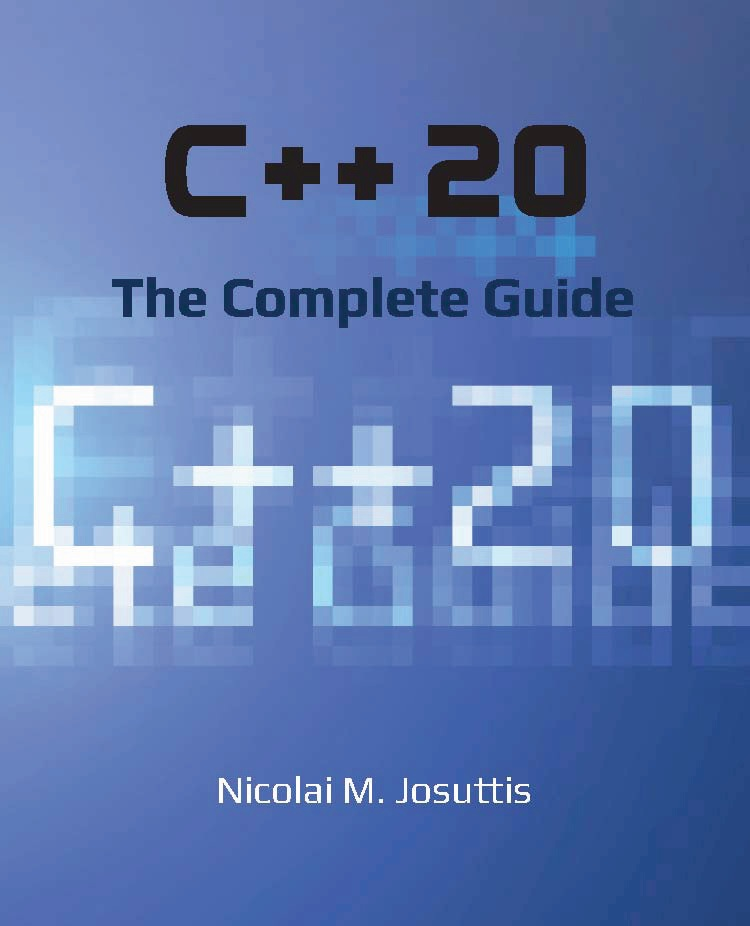
\includegraphics[width=\textwidth,height=\textheight,keepaspectratio]{cover.jpg}
			\begin{tikzpicture}[remember picture, overlay, inner sep=0pt]
				\node at (current page.center) 
				{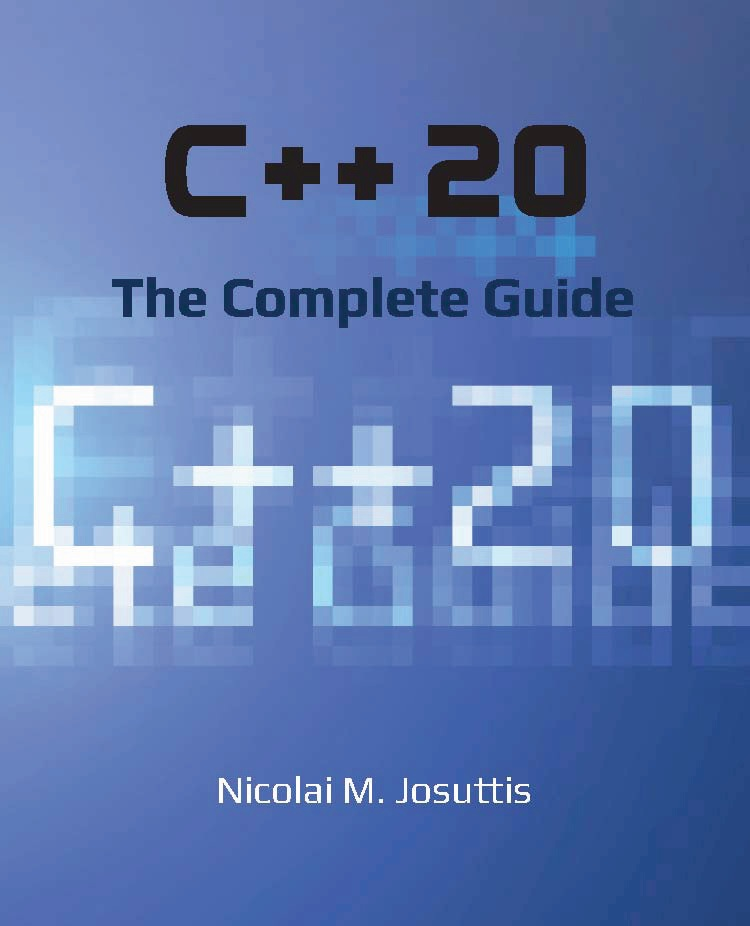
\includegraphics[width=\paperwidth, keepaspectratio=false]{cover.jpg}};
			\end{tikzpicture}
			\newpage
			\thispagestyle{empty}
			\huge
			\textbf{C++20 - The Complete Guide} 
			\\[9pt]
			\normalsize 
			作者: \href{http://www.josuttis.com/welcomee.html}{Nicolai M. Josuttis}
			\\[8pt]
			\normalsize
			译者:\href{https://github.com/xiaoweiChen/CXX20-The-Complete-Guide}{陈晓伟}
			\\[8pt]
			\normalsize 
			版本:\href{http://leanpub.com/cpp20}{2022-10-30}
		\end{center}
		
		\newpage
		
		\pagestyle{empty}		
		\tableofcontents
		\newpage
		
		\setsecnumdepth{section}
		
		\mySection{}{前言}{content/preface.tex}
		\newpage
		
		\mySection{}{关于本书}{content/chapter0/0.tex}
		\mySubsection{}{预备知识}{content/chapter0/1.tex}		
		\mySubsection{}{本书结构}{content/chapter0/2.tex}		
		\mySubsection{}{如何阅读}{content/chapter0/3.tex}		
		\mySubsection{}{执行方式}{content/chapter0/4.tex}		
		\mySubsection{}{C++标准}{content/chapter0/5.tex}		
		\mySubsection{}{示例代码和附加信息}{content/chapter0/6.tex}
		\mySubsection{}{反馈}{content/chapter0/7.tex}
		\newpage
		
		\mySection{第1章}{比较操作符<=>}{content/chapter1/0.tex}	
		\mySubsection{1.1.}{提出比较操作符<=>的动机}{content/chapter1/1.tex}
		\mySubsection{1.2.}{定义和使用}{content/chapter1/2.tex}
		\mySubsection{1.3.}{定义<=>和==操作符}{content/chapter1/3.tex}
		\mySubsection{1.4.}{重载解析与重写表达式}{content/chapter1/4.tex}
		\mySubsection{1.5.}{泛型代码中使用<=>}{content/chapter1/5.tex}
		\mySubsection{1.6.}{比较运算符的兼容性}{content/chapter1/6.tex}
		\mySubsection{1.7.}{附注}{content/chapter1/7.tex}
		\newpage
		
		\mySection{第2章}{函数参数的占位符类型}{content/chapter2/0.tex}
		\mySubsection{2.1.}{auto为普通函数参数}{content/chapter2/1.tex}
		\mySubsection{2.2.}{使用auto作为参数的实践}{content/chapter2/2.tex}
		\mySubsection{2.3.}{使用auto作为参数的细节}{content/chapter2/3.tex}
		\mySubsection{2.4.}{附注}{content/chapter2/4.tex}
		\newpage
		
		\mySection{第3章}{概念、需求和约束}{content/chapter3/0.tex}
		\mySubsection{3.1.}{提出概念和需求的动机}{content/chapter3/1.tex}
		\mySubsection{3.2.}{使用约束和概念}{content/chapter3/2.tex}
		\mySubsection{3.3.}{概念和约束在实践中的应用}{content/chapter3/3.tex}
		\mySubsection{3.4.}{语义约束}{content/chapter3/4.tex}
		\mySubsection{3.5.}{概念设计指南}{content/chapter3/5.tex}
		\mySubsection{3.6.}{附注}{content/chapter3/6.tex}
		\newpage
		
		\mySection{第4章}{详细介绍概念、需求和约束}{content/chapter4/0.tex}
		\mySubsection{4.1.}{约束}{content/chapter4/1.tex}
		\mySubsection{4.2.}{需求项}{content/chapter4/2.tex}
		\mySubsection{4.3.}{特别的布尔表达式}{content/chapter4/3.tex}
		\mySubsection{4.4.}{需求表达式}{content/chapter4/4.tex}
		\mySubsection{4.5.}{概念详解}{content/chapter4/5.tex}
		\mySubsection{4.6.}{使用概念作为类型约束}{content/chapter4/6.tex}
		\mySubsection{4.7.}{用概念包含约束}{content/chapter4/7.tex}
		\newpage
		
		\mySection{第5章}{详细介绍标准概念}{content/chapter5/0.tex}
		\mySubsection{5.1.}{所有标准概念的概述}{content/chapter5/1.tex}
		\mySubsection{5.2.}{语言相关的概念}{content/chapter5/2.tex}
		\mySubsection{5.3.}{迭代器和范围的概念}{content/chapter5/3.tex}
		\mySubsection{5.4.}{可调用对象的概念}{content/chapter5/4.tex}
		\mySubsection{5.5.}{辅助概念}{content/chapter5/5.tex}
		\newpage
		
		\mySection{第6章}{范围和视图}{content/chapter6/0.tex}
		\mySubsection{6.1.}{使用范围和视图}{content/chapter6/1.tex}
		\mySubsection{6.2.}{租借迭代器和范围}{content/chapter6/2.tex}
		\mySubsection{6.3.}{使用视图}{content/chapter6/3.tex}
		\mySubsection{6.4.}{销毁或修改范围的视图}{content/chapter6/4.tex}
		\mySubsection{6.5.}{视图和常量}{content/chapter6/5.tex}
		\mySubsection{6.6.}{视图分解容器的习惯用法}{content/chapter6/6.tex}
		\mySubsection{6.7.}{附注}{content/chapter6/7.tex}
		\newpage
		
		\mySection{第7章}{范围和视图的工具}{content/chapter7/0.tex}
		\mySubsection{7.1.}{范围作为视图的实用工具}{content/chapter7/1.tex}
		\mySubsection{7.2.}{新迭代器类别}{content/chapter7/2.tex}
		\mySubsection{7.3.}{新增迭代器和哨兵类型}{content/chapter7/3.tex}
		\mySubsection{7.4.}{处理范围的新函数}{content/chapter7/4.tex}
		\mySubsection{7.5.}{用于处理范围的新类型函数/工具}{content/chapter7/5.tex}
		\mySubsection{7.6.}{范围算法}{content/chapter7/6.tex}
		\newpage
		
		\mySection{第8章}{视图类型的详情}{content/chapter8/0.tex}
		\mySubsection{8.1.}{所有视图的概览}{content/chapter8/1.tex}
		\mySubsection{8.2.}{视图的基类和命名空间}{content/chapter8/2.tex}
		\mySubsection{8.3.}{外部元素的源视图}{content/chapter8/3.tex}
		\mySubsection{8.4.}{生成视图}{content/chapter8/4.tex}
		\mySubsection{8.5.}{过滤视图}{content/chapter8/5.tex}
		\mySubsection{8.6.}{转换视图}{content/chapter8/6.tex}
		\mySubsection{8.7.}{修改视图}{content/chapter8/7.tex}
		\mySubsection{8.8.}{多范围视图}{content/chapter8/8.tex}
		\newpage
		
		\mySection{第9章}{Span}{content/chapter9/0.tex}
		\mySubsection{9.1.}{使用Span}{content/chapter9/1.tex}
		\mySubsection{9.2.}{Span的缺点}{content/chapter9/2.tex}
		\mySubsection{9.3.}{Span的设计要点}{content/chapter9/3.tex}
		\mySubsection{9.4.}{Span的操作}{content/chapter9/4.tex}
		\mySubsection{9.5.}{附注}{content/chapter9/5.tex}
		\newpage
		
		\mySection{第10章}{格式化输出}{content/chapter10/0.tex}
		\mySubsection{10.1.}{格式化输出的例子}{content/chapter10/1.tex}
		\mySubsection{10.2.}{格式库的性能}{content/chapter10/2.tex}
		\mySubsection{10.3.}{格式化输出的详情}{content/chapter10/3.tex}
		\mySubsection{10.4.}{全局化}{content/chapter10/4.tex}
		\mySubsection{10.5.}{错误处理}{content/chapter10/5.tex}
		\mySubsection{10.6.}{自定义格式化输出}{content/chapter10/6.tex}
		\mySubsection{10.7.}{附注}{content/chapter10/7.tex}
		\newpage
		
		\mySection{第11章}{<chrono>的日期和时区}{content/chapter11/0.tex}
		\mySubsection{11.1.}{举例概述}{content/chapter11/1.tex}
		\mySubsection{11.2.}{基本计时概念和术语}{content/chapter11/2.tex}
		\mySubsection{11.3.}{基于C++20的Chrono扩展}{content/chapter11/3.tex}
		\mySubsection{11.4.}{I/O与Chrono类型}{content/chapter11/4.tex}
		\mySubsection{11.5.}{实践中使用Chrono扩展}{content/chapter11/5.tex}
		\mySubsection{11.6.}{时区}{content/chapter11/6.tex}
		\mySubsection{11.7.}{时钟的详情}{content/chapter11/7.tex}
		\mySubsection{11.8.}{Chrono的其他新功能}{content/chapter11/8.tex}
		\mySubsection{11.9.}{附注}{content/chapter11/9.tex}
		\newpage
		
		\mySection{第12章}{std::jthread和停止令牌}{content/chapter12/0.tex}
		\mySubsection{12.1.}{添加std::jthread的动机}{content/chapter12/1.tex}
		\mySubsection{12.2.}{停止来源和停止令牌}{content/chapter12/2.tex}
		\mySubsection{12.3.}{std::jthread的详情}{content/chapter12/3.tex}
		\mySubsection{12.4.}{附注}{content/chapter12/4.tex}
		\newpage
		
		\mySection{第13章}{并发特性}{content/chapter13/0.tex}
		\mySubsection{13.1.}{使用锁存器和栅栏的线程同步}{content/chapter13/1.tex}
		\mySubsection{13.2.}{信号量}{content/chapter13/2.tex}
		\mySubsection{13.3.}{原子类型的扩展}{content/chapter13/3.tex}
		\mySubsection{13.4.}{同步输出流}{content/chapter13/4.tex}
		\mySubsection{13.5.}{附注}{content/chapter13/5.tex}
		\newpage
		
		\mySection{第14章}{协程}{content/chapter14/0.tex}
		\mySubsection{14.1.}{什么是协程?}{content/chapter14/1.tex}
		\mySubsection{14.2.}{第一个协程示例}{content/chapter14/2.tex}
		\mySubsection{14.3.}{产生或返回值的协程}{content/chapter14/3.tex}
		\mySubsection{14.4.}{协程的Awaitable对象和Awaiter}{content/chapter14/4.tex}
		\mySubsection{14.5.}{附注}{content/chapter14/5.tex}
		\newpage
		
		\mySection{第15章}{协程详情}{content/chapter15/0.tex}
		\mySubsection{15.1.}{协程的约束}{content/chapter15/1.tex}
		\mySubsection{15.2.}{协程框架和promise}{content/chapter15/2.tex}
		\mySubsection{15.3.}{协程promise的详情}{content/chapter15/3.tex}
		\mySubsection{15.4.}{协程处理的详情}{content/chapter15/4.tex}
		\mySubsection{15.5.}{协程中的异常}{content/chapter15/5.tex}
		\mySubsection{15.6.}{为协程帧分配内存}{content/chapter15/6.tex}
		\mySubsection{15.7.}{co\_await和awaiter的详情}{content/chapter15/7.tex}
		\mySubsection{15.8.}{处理co\_await的其他方法}{content/chapter15/8.tex}
		\mySubsection{15.9.}{协程的并发使用}{content/chapter15/9.tex}
		\mySubsection{15.10.}{协程的特征}{content/chapter15/10.tex}
		\newpage
		
		\mySection{第16章}{模块}{content/chapter16/0.tex}
		\mySubsection{16.1.}{用例子说明添加模块的动机}{content/chapter16/1.tex}
		\mySubsection{16.2.}{具有多个文件的模块}{content/chapter16/2.tex}
		\mySubsection{16.3.}{实践中处理模块}{content/chapter16/3.tex}
		\mySubsection{16.4.}{模块的详情}{content/chapter16/4.tex}
		\mySubsection{16.5.}{附注}{content/chapter16/5.tex}
		\newpage
		
		\mySection{第17章}{Lambda的扩展}{content/chapter17/0.tex}
		\mySubsection{17.1.}{带模板参数的泛型Lambda}{content/chapter17/1.tex}
		\mySubsection{17.2.}{调用Lambda的默认构造函数}{content/chapter17/2.tex}
		\mySubsection{17.3.}{Lambda作为非类型模板参数}{content/chapter17/3.tex}
		\mySubsection{17.4.}{consteval的Lambda}{content/chapter17/4.tex}
		\mySubsection{17.5.}{对捕获的修改}{content/chapter17/5.tex}
		\mySubsection{17.6.}{附注}{content/chapter17/6.tex}
		\newpage
		
		\mySection{第18章}{编译时计算}{content/chapter18/0.tex}
		\mySubsection{18.1.}{关键字constinit}{content/chapter18/1.tex}
		\mySubsection{18.2.}{关键字consteval}{content/chapter18/2.tex}
		\mySubsection{18.3.}{constexpr函数的宽松约束}{content/chapter18/3.tex}
		\mySubsection{18.4.}{std::is\_constant\_evaluated()}{content/chapter18/4.tex}
		\mySubsection{18.5.}{在编译时使用堆内存、vector和字符串}{content/chapter18/5.tex}
		\mySubsection{18.6.}{其他constexpr扩展}{content/chapter18/6.tex}
		\mySubsection{18.7.}{附注}{content/chapter18/7.tex}
		\newpage
		
		\mySection{第19章}{非类型模板参数(NTTP)扩展}{content/chapter19/0.tex}
		\mySubsection{19.1.}{非类型模板参数的新类型}{content/chapter19/1.tex}
		\mySubsection{19.2.}{附注}{content/chapter19/2.tex}
		\newpage
		
		\mySection{第20章}{新类型特征}{content/chapter20/0.tex}
		\mySubsection{20.1.}{用于类型分类的新类型特征}{content/chapter20/1.tex}
		\mySubsection{20.2.}{用于类型检查的新类型特征}{content/chapter20/2.tex}
		\mySubsection{20.3.}{用于类型转换的新类型特征}{content/chapter20/3.tex}
		\mySubsection{20.4.}{新迭代器的类型特征}{content/chapter20/4.tex}
		\mySubsection{20.5.}{用于布局兼容性的类型特征和函数}{content/chapter20/5.tex}
		\mySubsection{20.6.}{附注}{content/chapter20/6.tex}
		\newpage
		
		\mySection{第21章}{核心语言的小改进}{content/chapter21/0.tex}
		\mySubsection{21.1.}{基于范围的for循环的初始化}{content/chapter21/1.tex}
		\mySubsection{21.2.}{using用于枚举值}{content/chapter21/2.tex}
		\mySubsection{21.3.}{将枚举类型委托给不同的作用域}{content/chapter21/3.tex}
		\mySubsection{21.4.}{新字符类型char8\_t}{content/chapter21/4.tex}
		\mySubsection{21.5.}{聚合的改进}{content/chapter21/5.tex}
		\mySubsection{21.6.}{新增属性和属性特性}{content/chapter21/6.tex}
		\mySubsection{21.7.}{特性测试宏}{content/chapter21/7.tex}
		\mySubsection{21.8.}{附注}{content/chapter21/8.tex}
		\newpage
		
		\mySection{第22章}{泛型编程的小改进}{content/chapter22/0.tex}
		\mySubsection{22.1.}{模板形参的类型成员的隐式类型名}{content/chapter22/1.tex}
		\mySubsection{22.2.}{泛型代码中聚合的改进}{content/chapter22/2.tex}
		\mySubsection{22.3.}{显式条件}{content/chapter22/3.tex}
		\mySubsection{22.4.}{附注}{content/chapter22/4.tex}
		\newpage
		
		\mySection{第23章}{C++标准库的小修改}{content/chapter23/0.tex}
		\mySubsection{23.1.}{字符串类型的更新}{content/chapter23/1.tex}
		\mySubsection{23.2.}{std::source\_location}{content/chapter23/2.tex}
		\mySubsection{23.3.}{整型值和大小的安全比较}{content/chapter23/3.tex}
		\mySubsection{23.4.}{数学常数}{content/chapter23/4.tex}
		\mySubsection{23.5.}{处理位的工具}{content/chapter23/5.tex}
		\mySubsection{23.6.}{<version>}{content/chapter23/6.tex}
		\mySubsection{23.7.}{算法的扩展}{content/chapter23/7.tex}
		\mySubsection{23.8.}{附注}{content/chapter23/8.tex}
		\newpage
		
		\mySection{第24章}{已弃用和已删除的功能}{content/chapter24/0.tex}
		\mySubsection{24.1.}{已弃用和删除的核心语言功能}{content/chapter24/1.tex}
		\mySubsection{24.2.}{已弃用和已删除的库功能}{content/chapter24/2.tex}
		\mySubsection{24.3.}{附注}{content/chapter24/3.tex}
		\newpage
		
		\mySection{}{术语表}{content/chapter25/0.tex}
		\mySubsection{}{A}{content/chapter25/1.tex}
		\mySubsection{}{C}{content/chapter25/2.tex}
		\mySubsection{}{F}{content/chapter25/3.tex}
		\mySubsection{}{G}{content/chapter25/4.tex}
		\mySubsection{}{I}{content/chapter25/5.tex}
		\mySubsection{}{L}{content/chapter25/6.tex}
		\mySubsection{}{P}{content/chapter25/7.tex}
		\mySubsection{}{R}{content/chapter25/8.tex}
		\mySubsection{}{S}{content/chapter25/9.tex}
		\mySubsection{}{U}{content/chapter25/10.tex}
		\mySubsection{}{V}{content/chapter25/11.tex}
		\mySubsection{}{X}{content/chapter25/12.tex}
		\newpage
		
	\end{sloppypar}
\end{document}

